\documentclass{utue} %utue.cls required for Uni Tuebingen corporate design
\usepackage[font=footnotesize,labelfont=bf]{caption}
\usepackage{hyperref}


% Values for title generation
\title{Reading scene text in deep convolutional sequences}
\author{Jan Haug, Marius Hobbhahn, Roman Schulte}
\date{\today}


% Subtitle is optional. It represents what kind of work you did.
\subtitle{Winter Term 2017}

\begin{document}
	


% You can place a teaser as follows. (Otherwise, just uncomment the following part)
\teaser{
    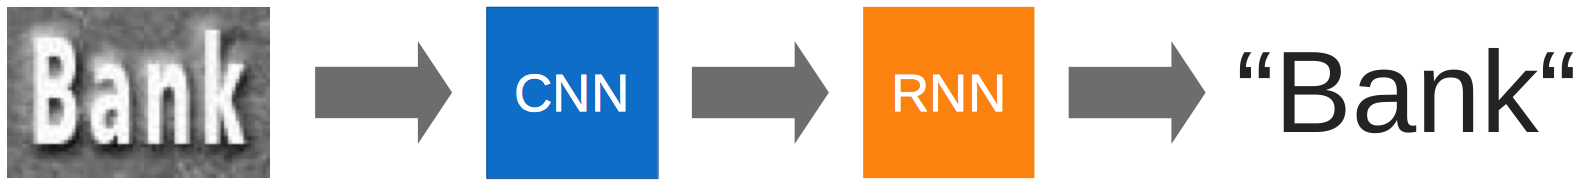
\includegraphics[width=\textwidth]{graphics/teaser}
    \caption{\label{fig:teaser}Basic concept of our network.}
}

% Creates title of document and additional title page.
\maketitle

\section*{Abstract}
The goal of our project was to implement a neural network which is able to identify text in real-world images.
Our work is based on He et. al ~\cite{2015arXiv150604395H}. The network consists of three parts: A CNN to detect major character features inside small slices of the image, an RNN to predict characters using the accumulated feature data and a CTC to reconstruct the final word. All parts were implemented using Python 3, the Tensorflow 1.6 API and some other supporting libraries. As in the original publication, we used the IIIT5K data set to train and test our network.

\section{Introduction}

Natural scene recognition is one of the most important tasks in numerous automation processes. Autonomous cars have to be able to identify construction signs to follow their instructions, traffic agencies can identify license plates of traffic offenders \cite{licenseplates} and robots will need to read text and numbers in a natural environment. In 2015, He et. al ~\cite{2015arXiv150604395H} proposed a model to read scene text in natural environments with a combination of a convolutional neural network (CNN) and recurrent neural network (RNN) which is not restricted to having words pre-defined in a dictionary or segmentation of individual letters (which poses a difficult task by itself), but instead views the input as a sequence and uses context information to decode a word as a whole, e.g. on an advertisement sign. One of the main challenges of scene recognition is the high variance in image quality and style of displayed signs. The same word can be represented in many different ways in an image by variation in lighting, colours, perspective or font. The approach chosen by the authors has some advantages over previous approaches (e.g. \cite{prevapproach1} \cite{prevapproach2}), which fail to capture all representations of strings in a natural environment. It uses a combined model, capitalizing on both the high performance in character recognition of CNNs and also the ability of RNNs to process context information in sequences. \\
\begin{enumerate}
	\item CNNs have become the de-facto state-of-the-art method for character recognition and to build high level representations of image data \cite{cnn1} \cite{cnn2} \cite{cnn3}.
	By moving a sliding window over a given picture, we are able to create character-level inputs without concerns about character segmentation, as this problem is handled by the RNN part of the model. The simplicity of a sliding window approach implies that some frames will not yield beneficial results, but the RNN is also able to process unclear outputs of the CNN; this only means that the sliding window should be moved in small steps, so no characters can be skipped by accident. On the other hand, this simplicity results in not only a small (i.e. fast) CNN, but also in a high versatility, as the inputs do not need to be pre-processed except for the trimming around a word and the re-scaling to a 32px height.
	\item RNNs are very strong at processing sequences of inputs and accounting for context information, especially when the length of a given sequence is unknown at first \cite{rnn1} \cite{rnn2}.\\
	As words are nothing else than sequences of letters (with variable length), the application of an RNN seems very intuitive. Due to this context information, the RNN can make decisions for a sign based on the previously identified signs, i.e. The letter 'a' might be more likely to occur after a 'b' than an 'y'. Since the RNN receives the activations of the penultimate layer of the CNN (which has more neurons), there should also be more information on letters in direct vicinity to the recognized one, since there will usually be more than one symbol in the sliding window. To use context information from previous and later signs we use a bidirectional approach, that independently applies the model forwards and backwards. 
	\item If property 1 and 2 are combined successfully, it is possible to process unknown words and arbitrary sequences of symbols. Since the training is done in a compositional way, it is independent of dictionaries or corpora of already known words and combinations of strings. Therefore it would be able to read the information on any given picture even if no meaning is attached to it. The only restriction is that the set of symbols needs to be specified as the CNN classifies each input as one of 26 letters or of the 10 different digits (i.e. the recognition of special letters like Umlauts would require slight modifications to the model and retraining it from scratch)
\end{enumerate}
The main contribution of this paper was to improve the accuracy in scene text recognition on given benchmark test sets like the IIIT5K~\cite{iiit5k}.
Our contribution is the attempt to reproduce the work of the paper, the comparison of the results given the same benchmarks, and the documentation of possible caveats or other difficulties during this process, especially where the authors do not specify details on the implementation or its parameters.

\section{Related Work}
%don't just copy papers from the original paper, but look for more recent ones, i.e. 2016/17
%describe the research goal of the other paper, the differences to our approach and why this difference is important here
% this is the citation of the main paper ~\cite{2015arXiv150604395H}
The paper in discussion was written by He et al. from 2015 ~\cite{2015arXiv150604395H}. In this section we would like to address two types of related papers. Firstly, papers that have tried different approaches to solve the same task but with less accurate results. These will be mainly papers published before the original paper. Secondly, we explore how the presented methods was applied to other related tasks in later publications. Follow up studies and improvements will be provided in the discussion part of this paper. \\
%papers before ours
Earlier approaches of text scene recognition like shown in ~\cite{iiit5k}, or ~\cite{6727574} used combinations of structure guided character recognition, linguistic knowledge and Bayesian inference via decision trees. All of these broke the benchmarks on frequently used data sets such as IIIT5K or ICDAR but did not use learning algorithms based on neural networks. First approaches of leveraging the advantages of neural networks were done for example by ~\cite{DBLP:journals/corr/AlsharifP13}, who used a classical CNN and hybrid hidden Markov models (HMMs), which could be seen as predecessors of the frequently used connectionist temporal classification (CTC) of today, which is also used in the final part of the model presented here.\\
%papers with different goal
The very same model idea as described here, i.e. a combination of sliding window, CNN, RNN and CTC, was used to significantly improve benchmarks for other tasks of scene recognition. ~\cite{DBLP:journals/corr/GuoTLL16} for example used the method for the recognition of house numbers and achieved an accuracy of 91 percent, compared to 81 percent of previous approaches. ~\cite{DBLP:journals/corr/LiS16} were able to lift the benchmark of license plate recognition on the Caltech cars data set from 95.5 to 97.56 and the recall from 84.8 to 95.24 percent. The difference between precision and recall in this paper not only implies superior recognition if the plate has been detected but also superior detection of license plates in the first place. Both of these papers show the strength of the combining CNN and RNN in a single model. The way~\cite{2015arXiv150604395H} differs from these approaches is through very high diversity of the image inputs: License plates and house numbers have much more structure and in the house number case, less different symbols on it. With the IIIT5K dataset, the network can make far fewer assumptions about its inputs, since there are a lot of different shapes within each class due to the vast amount of different fonts used.


\section{Structure of the network}

%just the theory behind the network
After applying a sliding window on a given image each frame is forwarded into a CNN. The sequence of resulting feature vectors is then fed as an input to the RNN which in turn outputs a sequence of characters and numbers. An overview of the whole network is given in figure~\ref{fig:model_general}.
\begin{figure}[h]
	\centering
	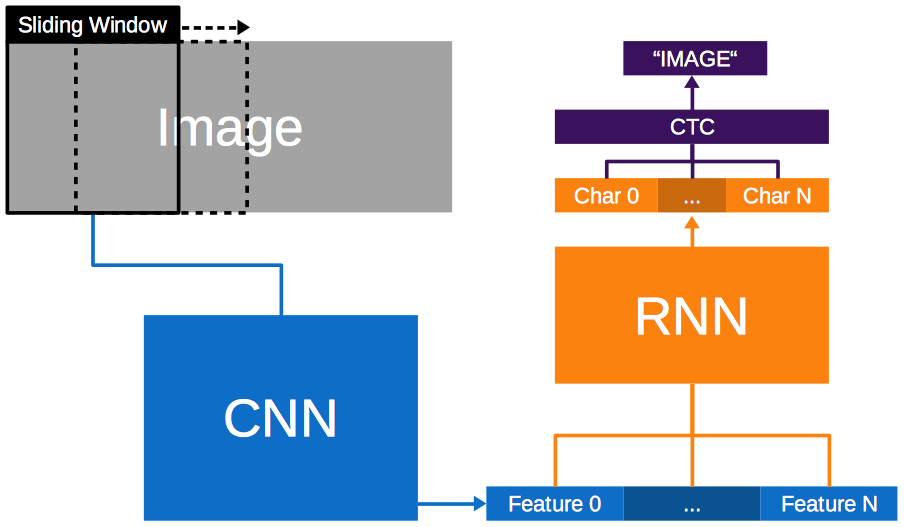
\includegraphics[width=.9\columnwidth]{graphics/model_general.png}
	\caption{\label{fig:model_general}General structure of the network.}
\end{figure}


\subsection{Data wrangling}
The IIIT5K provides 5000 real-world images each containing a single word. In general, this is exactly the type of data our network should handle. However, it is not possible to train the CNN with that kind of input, as it accepts needs $32\times32$ pixel images to learn single characters. These kind of data can be derived from the IIIT5K data set. Additionally to the labels the data set also provides some extra metadata about the data points. One of them are the bounding boxes of every character in the image. This information is used to create  new training and validation data sets based on the content of IIIT5K. The RNN expects a sequence of $128D$ feature vectors. Therefore, we created new data sets containing the output of the already trained CNN for every image of the IIIT5K. One thing we've noticed is a severe class-imbalance in the dataset, due to the fact that real-world examples use some letters like 'e' a lot more often than for example 'q'. This means, the CNN might be biased after training on this dataset and that it could lack generalization properties for some of the less common classes.
Outside of the training, our network can process any kind of image. When a image is passed to the network it will be preprocessed to match the requirements. This preprocessing includes: grayscaling, resizing and applying the sliding window.

\subsection{Structure of the CNN}
The CNN has 5 convolutional layers. In the first 3 we apply a 9x9 kernel on the inputs and use a max. group of 2. For the 4th layer a 8x8 kernel and a max group of 4 is used to reduce the dimensionality of the output vector to 128. Note that this output of a 128D feature vector is forwarded into the RNN, to provide more information than just hard class-probabilities. The 5th layer uses a 1x1 kernel %is this equivalent to no kernel? -- it means, it is fully connected ~Jan
(i.e. is fully connected) and afterwards applies a max group of 4 to further reduce dimensionality. This output is then forwarded through a fully connected layer with 36 outputs for the 26 possible characters and 10 numbers; note that the network does not distinguish between lower and upper case, but is trained on both versions of each letter. The ReLU function provides nonlinearity throughout the layers (next to the maxgrouping). Note that the last convolutional and the fully connected layer are merely used for the training of the CNN but later not used for the classification in the RNN. A detailed description of the network can be seen in graphic \ref{fig:cnn_structure}.

\subsection{Structure of the RNN}
The recurrent part of the network receives a sequence of feature vectors, each of which is provided by the CNN. We use bidirectional stacked long-short-term-memory (LSTM) cell blocks with 128 inputs respectively as developed by ~\cite{Hochreiter:1997:LSM:1246443.1246450} originally. Bidirectional means that the RNN essentially has 2 independent units. In one the sequence is put in forwards and the other backwards. The results are then concatenated afterwards and fed into a fully connected layer with 37 output classes. 26 for each character, 10 for numbers and 1 for undetectable sign or no character. This can be seen in figure \ref{fig:rnn_structure}. \\
\begin{figure}[h!]
	\centering
	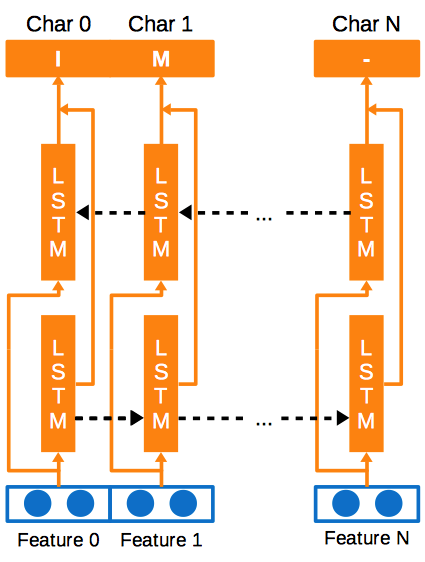
\includegraphics[width=.9\columnwidth]{graphics/model_rnn.png}
	\caption{\label{fig:rnn_structure} Structure of the RNN with a bidirectional approach with 128 inputs respectively.}
\end{figure}

% Moved cnn figure here for better layout
\begin{figure*}[h!]
	\centering
	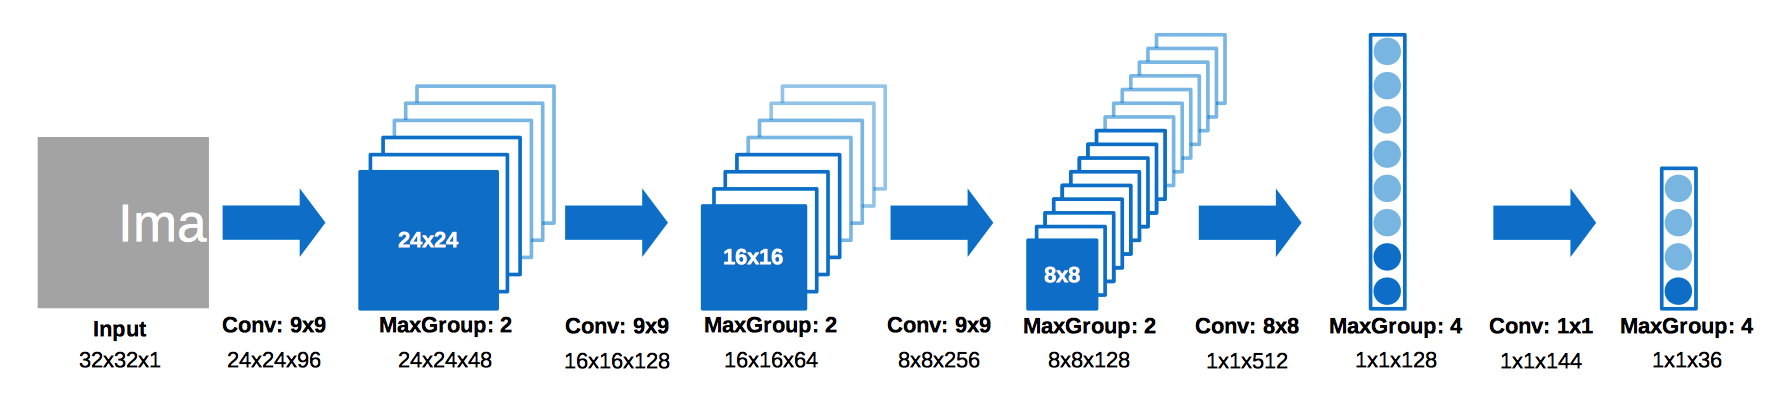
\includegraphics[width=\textwidth]{graphics/model_cnn.png}
	\caption{\label{fig:cnn_structure} Structure of the CNN with 5 convolutional and 5 grouping layers.}
\end{figure*}

At this point we still have redundancies or unclear information due to the sliding window, as we cannot know in advance the optimal step size for a given input image (i.e. how  many characters it contains). To solve this problem, "connectionist temporal classification" (CTC) is used. A detailed explanation would be outside of the scope of this paper and can be found in the original paper  ~\cite{Graves:2006:CTC:1143844.1143891}.
For the purpose of this paper, one may consider it as a way to remove unlikely and redundant information given the labels. In sequential information the placement of non-character symbols or redundancies is always hard to deal with. The CTC approach therefore uses a hidden Markov model (HMM) to sample different possible outcomes as paths in a tree and choose the path with the highest likelihood. Consider an example where the sequence after the LSTM cell block is "iiii---mmmmaaagggee--", where '-' represents the non-character symbol. The CTC would then reduce the redundancies and remove non-character symbols until the most likely outcome, "image" is put out. The information learned by the CTC during the training are backpropagated through the network such that future classification can already access them. A graphical overview is provided in figure \ref{fig:structure_ctc}. \\
\begin{figure}[h!]
	\centering
	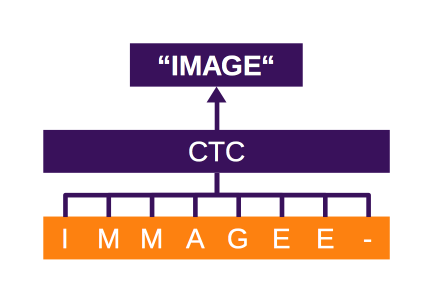
\includegraphics[width=\columnwidth]{graphics/model_ctc.png}
	\caption{\label{fig:structure_ctc} Simplified structure of the CTC.}
\end{figure}

\section{Implementation details}
%here are the names of functions, comparisons with other possible implementations and numbers (i.e. number of epochs, momentum terms, learning rates, etc. )
The project is written in Python 3. It uses the Tensorflow 1.6 API to build and train the network graph. Other libraries we used are: Tensorpack (0.8.5), which simplifies the usage of Tensorflow for maschine learning, OpenCV for image processing and Numpy as a math framework.

\subsection{Data wrangling}
One of the major challenges in this project was to setup the data flow. As Python is an untyped language, it is easy to pass the right data in the wrong format. Sometimes this does not lead to a runtime error, but to useless training results. As an example, we expected the grayscaled image to be a 32x32 image of floating point numbers ranging from 0 to 1 (i.e. the usual representation). To center the image around zero, we multiplied by 2 and subtracted 1. However, a while later we discovered that the inputs were actually integers ranging from 0 to 255, which we then had shifted to $[-1, 509]$ instead, producing very large activations within the network.

\paragraph{Image preprocessing}
The CNN expects the input images to have a size of $32\times32$ pixels and only a single color channel. Most real world images will not match this requirements. Therefore we need to transform the input images and feed them in small bites to the CNN. The first step of the preprocessing merges all color channels of the input image into one. After that we resize the image to a height of 32 pixels, but keeping the aspect ratio. Now we can apply the sliding window and pass a small sub-image (i.e. a 32px wide slice) to the CNN. After each step, the sliding window is moved 8 pixels until it reaches the end of the image. Figure \ref{fig:sliding_window} shows an example for this step.

\begin{figure}[h!]
	\centering
	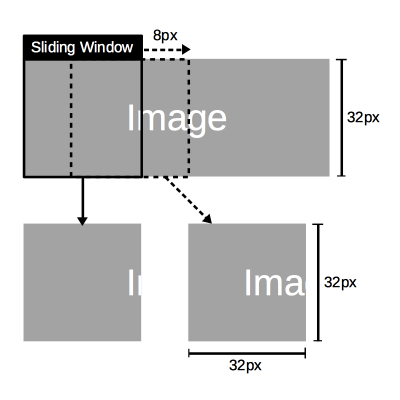
\includegraphics[width=\columnwidth]{graphics/model_sliding_window.png}
	\caption{\label{fig:sliding_window} Graphical depiction of the sliding window.}
\end{figure}


\paragraph{RNN training data}
One major problem in training the RNN was to provide the labels for a batch. The CTC expects the labels of one batch to share the same length, which does not match the desired use case, as we do not know the word or its length in advance. Therefore, the labels need to expanded to have the same length. This is done by determining the maximal label length in each batch and then padding the other labels to the same length. This is implemented by using a sparse tensor, where empty entries represents the non-character symbol. Figure \ref{fig:impl_rnn_labels} shows a example with a batch size of 4.

\begin{figure}[h!]
	\centering
	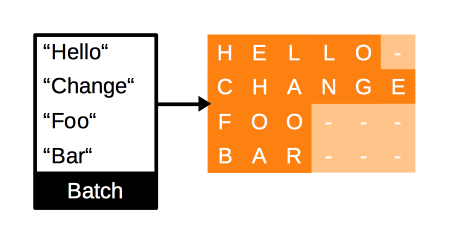
\includegraphics[width=.9\columnwidth]{graphics/impl_rnn_labels.png}
	\caption{\label{fig:impl_rnn_labels} Implementation of label batches.}
\end{figure}


\subsection{Implementation details of the CNN}
The convolutional layer were implemented using the \texttt{conv2D()} function provided by the Tensorpack library and combined with a self-made \texttt{maxgroup()} function, since the tensorflow version had an error. The functionality of the maxgroup can be seen in figure \ref{fig:impl_maxgroup}. The layers all use the ReLU activation function, for training we used an additional fully connected layer with the identity activation to output the probabilities for the 36 labels. \\
\begin{figure}[h!]
	\centering
	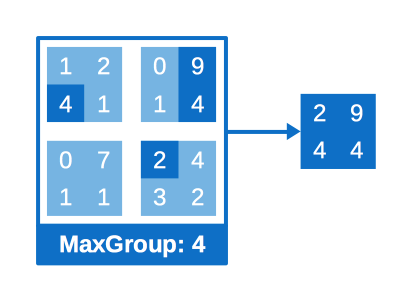
\includegraphics[width=.9\columnwidth]{graphics/impl_maxgroups.png}
	\caption{\label{fig:impl_maxgroup} Example of a MaxGroup with group size 4. Essentially Max-Pooling in the "Channel" dimension}
\end{figure}

For the training, we use a learning rate with exponential decay starting at 0.001 with decay rate of 0.99 and getting smaller every 5 epochs. As an optimizer, we chose the \texttt{AdamOptimizer()} after~\cite{Adam} and used the prebuilt \texttt{InferenceRunner()} from tensorpack to check for validation accuracy on a test set and prevent overfitting. In total, we trained for 1500 epochs and use the prebuilt \texttt{SimpleTrainer()} from tensorpack.


\subsection{Implementation details of the RNN}
The RNN is implemented using the prebuilt tensorflow functions \texttt{tf.nn.bidirectional\_dynamic\_rnn} with \texttt{tf.nn.BasicLSTMCell} for both directions. We use 128 LSTM units (see~\cite{lstmpaper}) as described in the original paper and the default for LSTMs - tanh (\textit{tangens hyperbolicus}) - as activation function. The final output of the RNN in each step (of the sequence) is computed by a fully connected layer mapping the LSTM outputs to the 37 class labels.
%this text is really redundant so far %besser? ~Jan
The CTC exists prebuilt as well. For the loss we use the \texttt{tf.nn.ctc\_loss} and \texttt{tf.nn.ctc\_greedy\_decoder} for the model. The greedy decoder is a variant of the \texttt{tf.nn.ctc\_beam\_search\_decoder} function that is faster but less accurate. For our training, the beam search decoder was too slow and in comparison did not add any visible improvements during the first couple of steps in training which lead us to using the greedy decoder. The beam search decoder can however be used at test time to improve accuracy\\
For the training we again use the Adam optimizer with a learning rate of 1e-4 and a momentum term of 0.9 over 1500 epochs. Since we divided our data set in test and train split, we also use the \texttt{InferenceRunner()} class provided by the tensorpack library to reduce overfitting and check for validation accuracy. 

\subsubsection{Ensembling}
In an attempt to improve accuracy, we tried using an ensemble of CNNs to provide more features for the RNN. Ensembling is a common technique used to reduce the variance of neural networks and improve generalization \cite{ensembles}. The CNN implementation is not affected by this, as the training process was just repeated 3 times to create independent models.\\
For the RNN, we created a new training class which accepts several model paths (one could also use more than 3 models with this implementation at the cost of computational resources). Then, a FeaturePredictor is initiated for every stored model and their results are concatenated into a vector with $(128\cdot num_models)$ features which are then fed into the RNN.

\section{Experiments and Results}
%detailed description of what datasets we were using, what the results of the singular training for the CNN were, what the results for the RNN were
%explanation of the inference runner, test error and validation accuracy
The test images solely came from the openly available IIIT5K data set. In the original study, two other sets of images were additionally used but seemed to only contribute very small amounts of images. So only using the IIIT5K seemed sufficiently justifiable in this case. As the name suggests we initially have 5000 images of which a small amount was sorted out since they did not have 32 pixels in width. After segmentation the CNN trains on %insert number of labeled 32x32 pictures
labeled $32\times32$ pictures and the RNN on around 2500 pictures with scene text due to the test train split and since we sorted out images which didn't fit at least as many sliding windows (with the respective step size) as there are characters. For example, while an image with size 38x32 is large enough for character recognition, it does not fit enough slices for a word with 3 or more characters.\\
The experiments were conducted on the data sets described above using the training details listed in the respective implementation details section. \\
The CNN converges against an accuracy of 0.97 on the training set with a validation accuracy of 0.62. The process can be viewed in figure~\ref{fig:cnn_accuracy}.\\

\begin{figure}[h!]
	\centering
	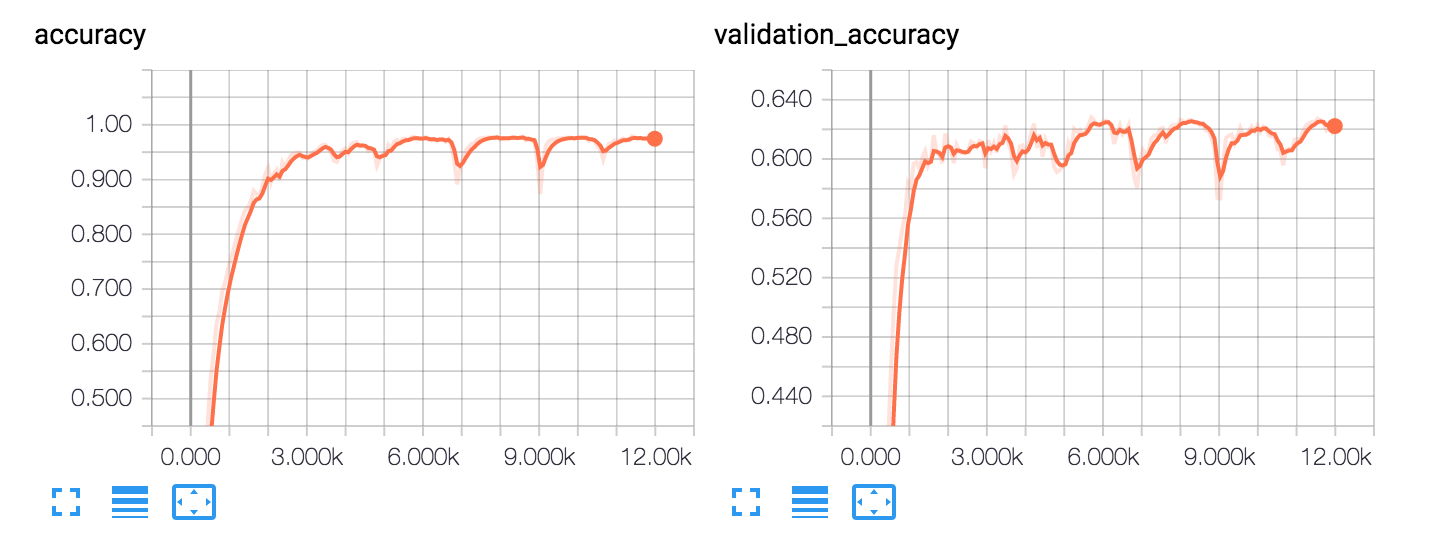
\includegraphics[width=\columnwidth]{graphics/cnn_accuracy.png}
	\caption{\label{fig:cnn_accuracy}Training process for the CNN. Training accuracy on the left and validation accuracy on the right.}
\end{figure}

The validation accuracy seems rather low for a task like character recognition. This might be due to overfitting, very unclear images or just a suboptimal model. But note that the 5th and 6th layer of the CNN never get used at later stages anyways so only the accuracy of the 128D feature vectors (which still contain more information) matters. This cannot be determined directly but only through the loss of the RNN at later stages. \\
Generally, the CNN's architecture seems rather unconventional, as it uses large kernels without padding and uses maxout instead of maxpooling; maybe the authors try to "focus" the network on each images center as there can be multiple characters within one sliding window. However, we tried "ResNet" \cite{resnet1}, a more sophisticated architecture to compare against the CNN of \cite{2015arXiv150604395H}. The implementation follows \cite{resnet2} and was taken from \cite{tensorpack} with some modifications to use the IIIT5K dataset. As shown in figure~\ref{fig:resnet}, the results outperform our version of the CNN, cutting the remaining validation error in half, even without fine tuning of hyper-parameters (we only reduced the training length by a factor of 4 to account for the smaller dataset)
\begin{figure}[h!]
	\centering
	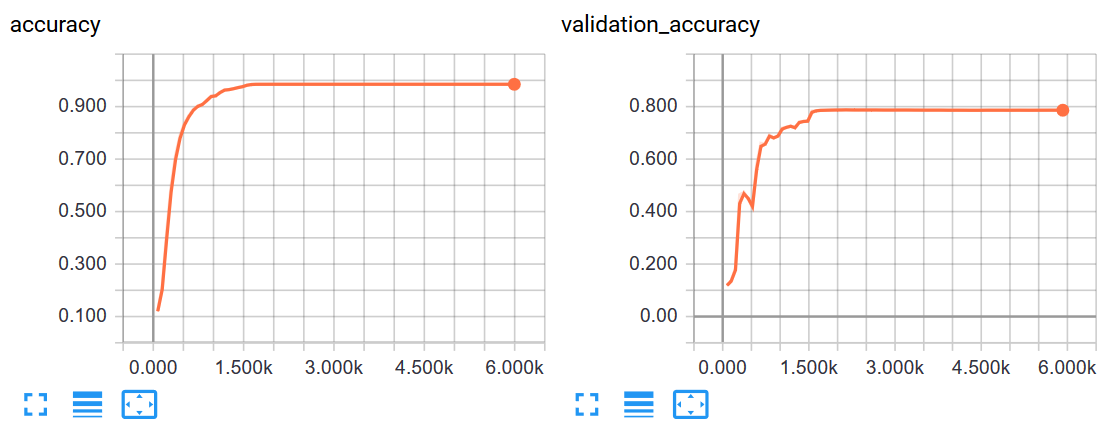
\includegraphics[width=\columnwidth]{graphics/resnet_accuracy.png}
	\caption{\label{fig:resnet}Training process for the residual network (ResNet). Training accuracy on the left and validation accuracy on the right.}
\end{figure}

The RNN converges against an accuracy of 1 on the training set and achieves a validation accuracy of $0.68$ before it begins to overfit. Note here that this is an increase compared to the 0.62 of the CNN itself, suggesting the context of the word significantly added to identification of the letters. Additionally, most words that are not correctly identified are only one letter off, which suggests that the RNN's accuracy would be a lot higher if we used character distance as an accuracy measure. For example the word "wraps" was identified as "wras" and "chandigarh" became "chandgarh".%maybe add graphic for these examples
The whole training process is seen in figure \ref{fig:rnn_accuracy}. It might be possible to improve validation accuracy by adding more regularization techniques (and by using more data).

\begin{figure}[h!]
	\centering
	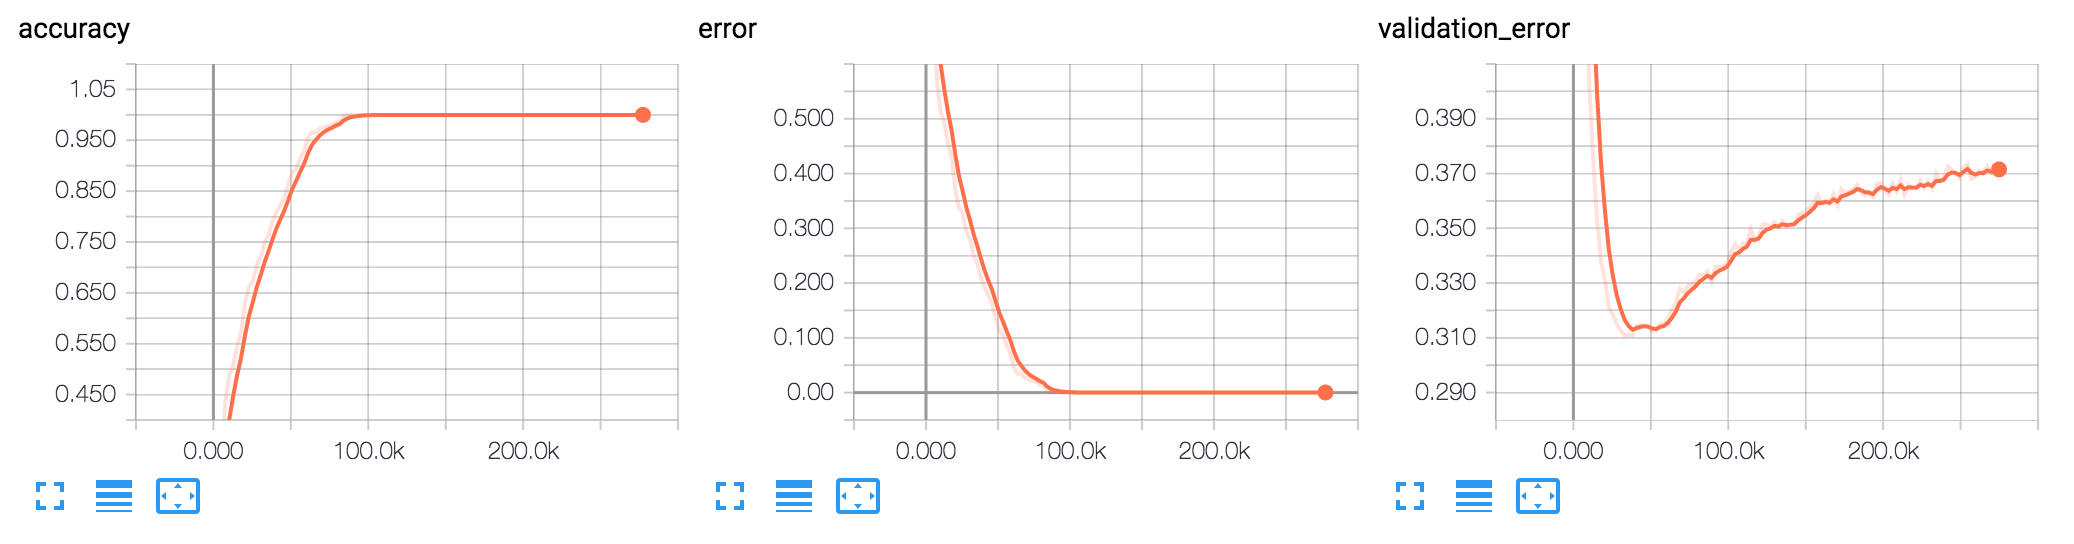
\includegraphics[width=\columnwidth]{graphics/rnn_accuracy.png}
	\caption{\label{fig:rnn_accuracy} Training process for the RNN. Training accuracy on the left, error in the center and validation error on the right.}
\end{figure} 
One thing we tried is using a CNN ensemble, i.e. separately training 3 CNNs and concatenating their 128D feature-vectors to provide a larger input with more information to the RNN. While the CNNs used for the ensemble achieved only between $0.51$ and $0.56$ validation accuracy, this improved the RNN to $\sim 0.72$, suggesting that this technique could be used to boost the model's results for high-performing CNNs as well. The training process of the 3 CNNs is displayed in figure~\ref{fig:cnn_ensemble} while the RNN's error is graphed in figure~\ref{fig:rnn_ensemble}

\begin{figure}[h!]
	\centering
	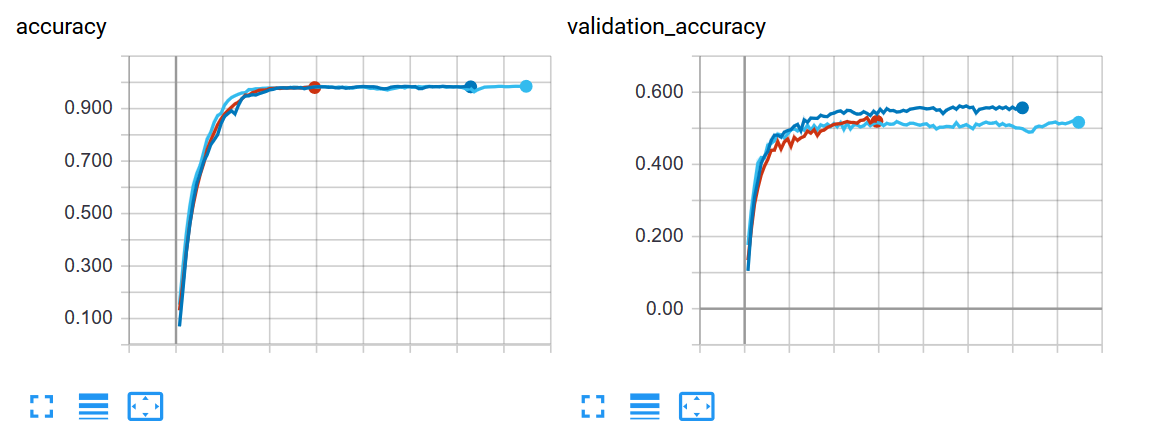
\includegraphics[width=\columnwidth]{graphics/cnn_ensemble_accuracy.png}
	\caption{\label{fig:cnn_ensemble} Training process for the CNNs used in the ensemble. Training accuracy on the left and validation accuracy on the right.}
\end{figure} 
\begin{figure}[h!]
	\centering
	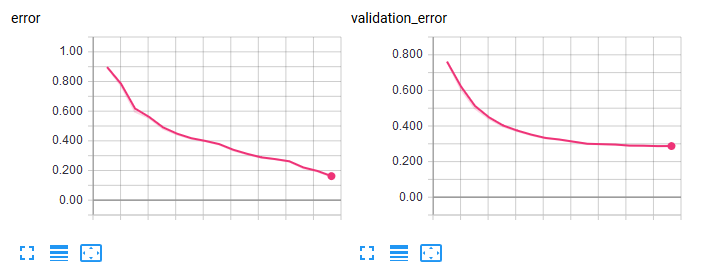
\includegraphics[width=\columnwidth]{graphics/rnn_ensemble_accuracy.png}
	\caption{\label{fig:rnn_ensemble} Training process for the RNN built on top of the ensemble. Training error on the left and validation error on the right.}
\end{figure} 

In comparison to the original, however, our results are rather unspectacular. Their accuracy was between 91,5 and 94 percent for the IIIT5K data set and even identified very ambiguous pictures. This difference could be caused by a number of reasons. First, they used additional datasets, which not only increases the amount, but also the diversity of the data, leading to better generalization properties. This applies to both CNN and RNN additively, as the better CNN also improves the limit of what the RNN can do. Then, the authors of the paper might have discovered some better hyper-parameter settings which were not explicitly mentioned in the publication, for example initialization variance and bias for the weights or the RNN's step size. Finally, they could have artificially extended their dataset with data augmentation (at least for the CNN training) by means such as random cropping or color scaling.

\section{Conclusion}
%include ideas that could further improve the accuracy, i.e. not train in two steps but in one, use other datasets as well, smaller step sizes for sliding window
%name other papers that are related to this or follow up on it (and what they did better)
The results that we achieved where slightly less impressive than those of the original publication. However, as explained above, there are a number of factors where our implementation could be improved in every step. The dataset used in training is relatively small compared to some other sets (e.g. MNIST), especially considering that IIIT5K contains highly different representations of each one. The generalization properties could be improved by adjusting the bias caused by the class imbalance in the dataset. The CNN and RNN both could be configured more optimally. One could also try propagating the RNNs error into the CNN, i.e. continue to adjust the CNNs weights during RNN training instead of completely separating the training process.\\
Even small improvements in generalization, especially on character recognition level could increase the accuracy by a lot, since most "wrong" results are already very close to the actual label.\\
Also, while the architecture of the CNN is unconventional, it is probably inferior to modern classification architectures. As shown above, a ResNet \cite{resnet1} achieves much higher accuracy (with less fine-tuning), other state-of-the-art architectures used in classification might lead to an even larger boost. As the RNN's false predictions are usually only off by one character, even moderate improvements in the CNN could lead to a significantly higher performance of the final model.\\
Ensembling shows some improvements over single CNNs as expected, this could also be applied to the modern architectures, especially if they are kept computationally efficient.
%%am stück trainieren kommt mir sehr schwierig vor, das könnte extrem lange brauchen, bis man den fehler durch eine ganze sequenz und das RNN zurückpropagiert hat. pre-training vom CNN wird notwendig sein, allerdings könnte man im RNN training die fehler ins CNN weiterpropagieren ~Jan
%There are a couple of improvements that could be done in future research projects that we would like to outline. A first idea would be to train the network not in 2 separate steps but rather as one end-to-end process. This would likely result in better outcomes since the entire CNN would already get information from the RNN and CTC through backpropagation. A second idea is to use a bigger data set of images for training. The IIIT5K seems like a good benchmark but due to the test train split, overfitting might have occured which might be solved by significantly bigger datasets. A third possibility is to train the CNN and RNN on significantly lower sliding window frame sizes, i.e. 2 instead of 8 %actually we are doing this. 
\\
The paper we are replicating was published in summer 2015 which is already two and a half years back. In a field with such rapid changes like scene recognition, other projects have already further improved the methods that were revolutionary then. In the following we would like to have a closer look at some of the new ideas and improvements. \\
%read and cite the followup paper
The first improvements were made by~\cite{DBLP:journals/corr/abs-1709-01727} who improved the sliding window by constructing it in a way that more closely resembles the movements of saccades by our eyes. They also added more layers to the CNN in the first step of the training. Lastly, they improve the CTC algorithm to reduce the search space and make training with a beam decoder more effective. In the end they were able to improve accuracy from 94 to 98.9 and 91.5 to 96.7 percent on the IIIT5K dataset respectively. 
The second paper by~\cite{DBLP:journals/corr/TianHHH016} is one conducted by partly the same authors that uses a similar approach to the original but contributed a new method which they call connectionist text proposal network (CTPN). The CTPN essentially is a convolutional network that already detects text structures within bigger image scenes. Due to this new technique they were not only able to find text within natural images, without cutting it out manually as in our paper, but also significantly improve nearly all benchmarks on the ICDAR data sets from 2011, 2013 and 2015.
%find and compare to other approaches
The last paper uses a slightly different approach on the just named ICDAR data sets. In~\cite{DBLP:journals/corr/HeH0Y15}, they only use a text-attentional convolutional neural networks for scene text detection without any recurrent part. They were able to break the benchmark of the ICDAR 2013 data set but were very quickly beaten afterwards by~\cite{DBLP:journals/corr/TianHHH016} which uses an RNN. However, it still goes to show that there still exist potent methods for text classification which do not require a recurrent part.\\


\bibliographystyle{alpha}
\bibliography{bibliography}
%https://github.com/chongyangtao/Awesome-Scene-Text-Recognition
%https://arxiv.org/abs/1709.01727 (this is a follow up paper)
%https://arxiv.org/pdf/1601.01100.pdf (same approach for house number recognition)
%http://adsabs.harvard.edu/abs/2016arXiv160105610L (same approach for license plate recognition)

\end{document}
